\subsection{Partial residual and added-variable plots}\label{sec:logist-partial}
The graphical methods described in this section are relatively
straight-forward indicators of the adequacy of a particular model,
with a specified set of predictors, each expressed in a given way.
More sophisticated methods have also been proposed, which focus on the need to include a particular predictor and whether its relationship is linear.
These include the \glossterm{partial residual plot},
\glossterm{added-variable plot}, and the
\glossterm{constructed variable plot},
which are all analogous to techniques developed in OLS.

\subsubsection{Partial residual plots}
The partial residual plot \citep{LarsenMcCleary:72} is designed to
show whether a given variable, $x_j$, included linearly in the model,
actually shows a nonlinear relation, requiring transformation.
As adapted to logistic regression by \citet{Landwehr-etal:84},
the partial residual for variable $x_j$ is defined as
\begin{equation*}%\label{eq:partres}
\vec{r}^{\star} = \mat{V}^{-1} \vec{r} + \beta_j \vec{x}_j
 = \frac{\vec{y} - \vec{p}}{ \vec{p} (1 - \vec{p})} \period
\end{equation*}
The partial residual plot is then a plot of $\vec{r}^{\star}$ against
$\vec{x}_j$, possibly with the addition of a smoothed lowess curve
\citep{Fowlkes:87} and
a linear regression line to aid interpretation.
If $x_j$ affects the binary response linearly, the plot should be approximately linear with a slope approximately equal to $\beta_j$.
A nonlinear plot suggests that $x_j$ needs to be transformed, and
the shape of the relation gives a rough guide to the required
transformation.
For example, a parabolic shape would suggest a term in $x_j^2$.

\subsubsection{Added variable plots}
The added variable plot, developed for generalized linear models by
\citet{WangP:85}, is a diagnostic plot designed to indicate whether
some new regressor, $z$, should be added to the model
which includes other explanatory variables.
An overall test could be based on the difference in $G^2$ for
the enlarged model $\logit(\vec{p}) = \mat{X} \vec{\beta} + \gamma \vec{z}$,
compared to the reduced model
$\logit(\vec{p}) = \mat{X} \vec{\beta}$.
But the added variable plot shows whether the evidence for including
$z$ is spread throughout the sample or confined to a small subset
of observations.
The regressor $z$ may be a new explanatory variable, or a higher power
of a variable already in the model.

The added variable plot may be constructed by following the logistic
regression for the reduced model with the variables in $\mat{X}$
with one weighted least squares regression of $\vec{z}$ on
$\mat{X}$ to find the residual part, $z^{\star}$,  of $z$ not predicted
by the previous regressors.
Let $\vec{r}$ be the vector of Pearson residuals from the initial logistic
fit of $\vec{y}$ on the variables in $\mat{X}$,
and let $\mat{H}$ and $\mat{V} = \diag [ \hat{\vec{p}} ( 1 - \hat{\vec{p}})]$
be the hat matrix and V matrix from this analysis.
Then, the added variable plot is a \scat\ of
the residuals $\vec{r}$ against the $z$-residuals,
\begin{equation*}%\label{eq:addvar}
 \vec{z}^{\star} = ( \mat{I} - \mat{H} ) \mat{V}^{1/2} \vec{z} \period
\end{equation*}
The $z$-residuals are easily calculated as
$z_i^{\star} = ( z_i - \hat{z}_i ) \sqrt{v_{ii}}$,
where $\hat{z}_i$ is the fitted value of $z_i$
in a weighted least squares regression of $\vec{z}$ on $\mat{X}$
using the $v_{ii}$ as weights.

A linear relation in this plot indicates that $z$ should be included in the
model, but observations with extreme $z$-residuals would be highly
influential in this decision.  A line fitted to this plot should have
an intercept approximately zero, and a slope approximating the coefficient
$\gamma$ of $z$ in the full model.
Added variable plots are produced by the \macro{ADDVAR}, described
in \macref{mac:addvar} and illustrated in the following example.

\begin{Example}[icu3]{Survival in the ICU}
In \exref{ex:icu1} we saw that the backward selection method nominated
three other variables, Systolic, pH, and PCO in addition to the four
variables we have been using throughout.
Here we first investigate whether systolic (blood pressure) should be
added to the model which includes Age, Admit, Cancer and Uncons.

The \macro{ADDVAR} is called as follows, to produce \figref{fig:icu61}.
There is no evidence of a strong linear relation, suggesting that
Systolic blood pressure has only a weak relationship to the residual in the current model.  The smooth lowess curve suggests
that any relationship may
be mildly quadratic
(though partial residual plots are generally preferable for detecting
nonlinearity).
The labeled points are those whose studentized Pearson residuals
exceed 2 in absolute value.
\begin{listing}
%addvar(data=icu,
   y=Died,                       /* response */
   x=age admit cancer uncons,    /* original predictors */
   z=Systolic,                   /* added variable */
   id=patient,                   /* id variable */
   smooth=0.5);                  /* lowess smoothing fraction */
\end{listing}

\begin{figure}[htb]
  \centering
  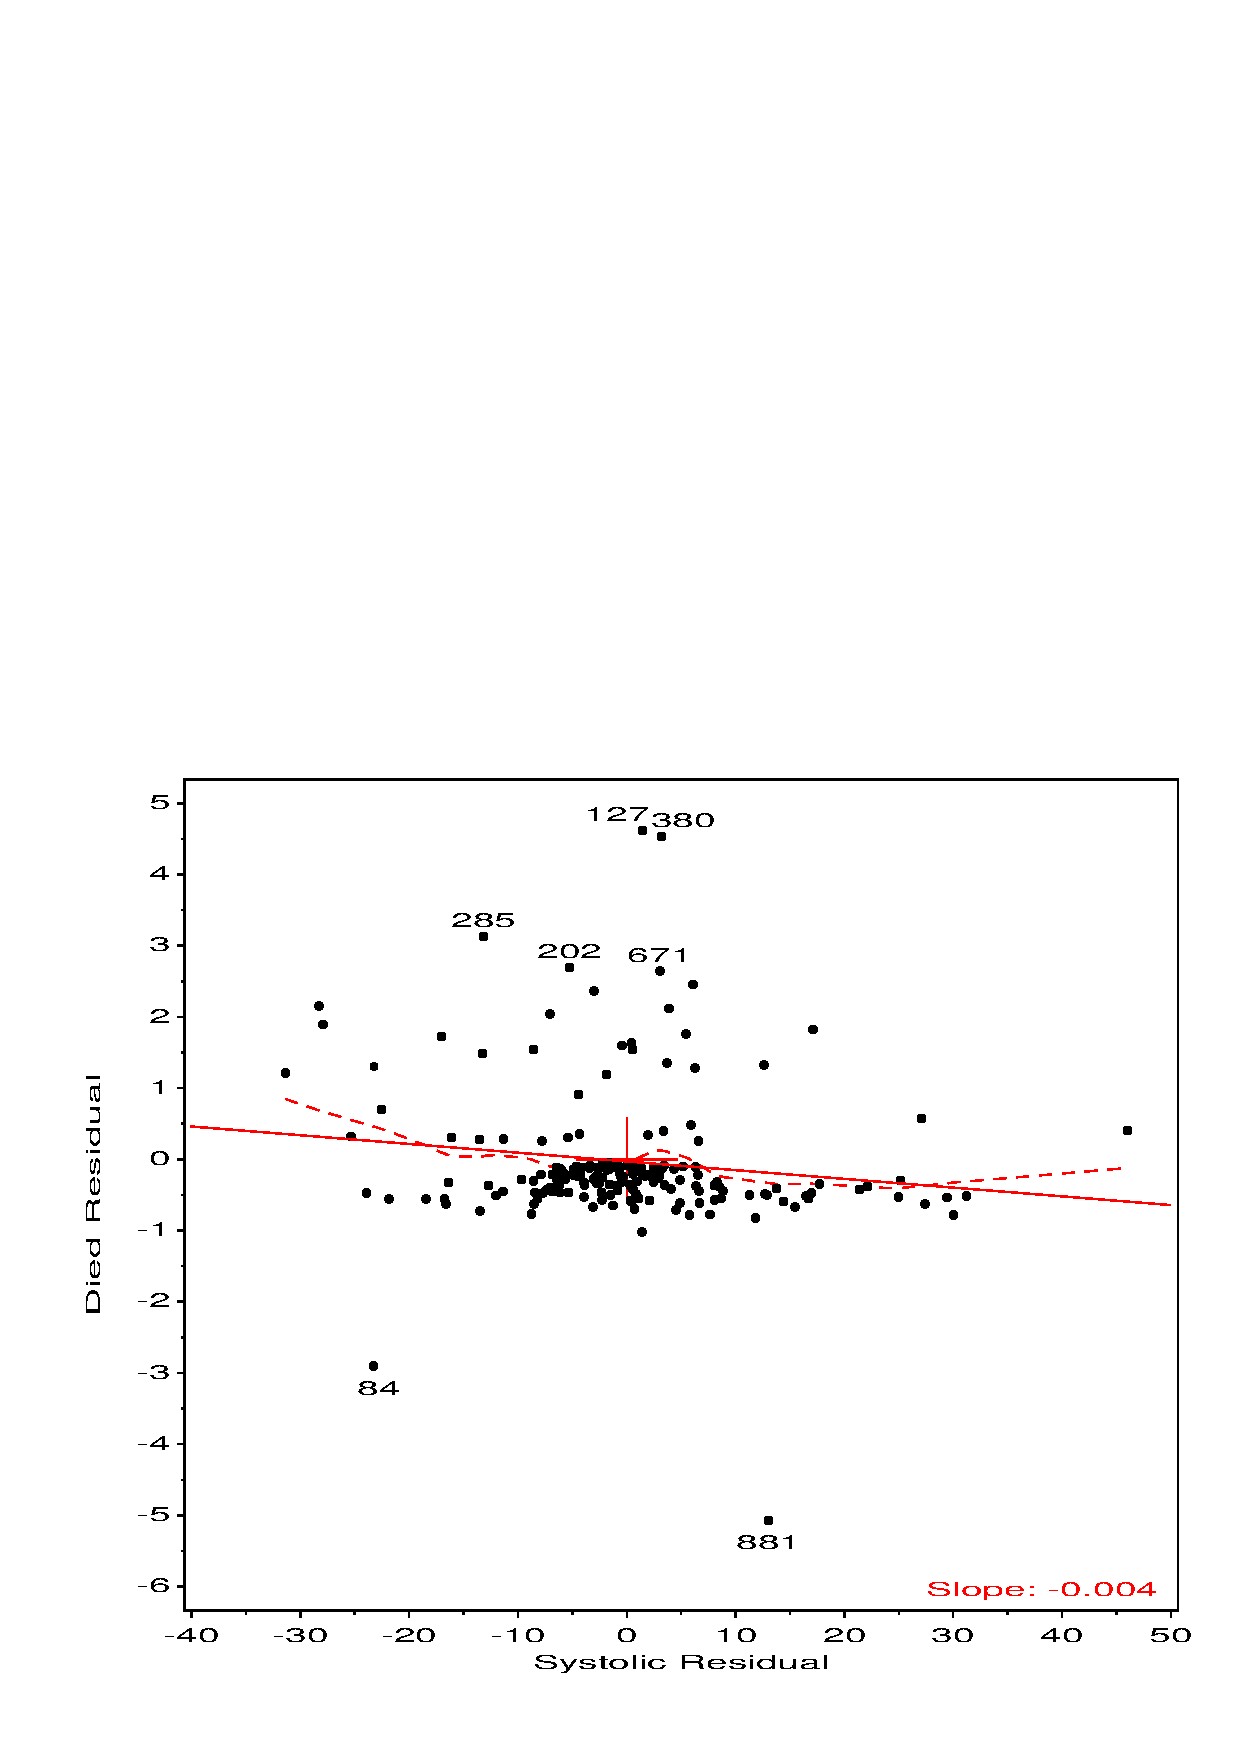
\includegraphics[scale=.6]{ch6/fig/icu61}
  \caption[ICU data: Added variable plot for Systolic blood pressure]{ICU data: Added variable plot for Systolic blood pressure.
 The solid line shows the weighted least squares regression of residuals
 on the Systolic residuals.  The broken curve is the lowess smooth.}%
  \label{fig:icu61}
\end{figure}

The added variable plot may also be used to determine if a regressor
should be included with an additional polynomial term.
For example we might check to see if Age${}^2$ should be included
in the model.  The statements below produce \figref{fig:icu62}.
\begin{listing}
data icu;
   set icu;
   age2 = .01 * (age-57.5)**2;

%addvar(data=icu, y=Died,  x=age admit cancer uncons, z=Age2,
   id=patient, smooth=0);
\end{listing}

%% one figure
\begin{figure}[htb]
  \centering
  \includegraphics[scale=.6]{ch6/fig/icu62}
  \caption{ICU data: Added variable plot for Age${}^2$}%
  \label{fig:icu62}
\end{figure}
The slope of the line in \figref{fig:icu62} is approximately zero,
so we conclue that the squared term in Age is unnecessary.
\end{Example}

\subsubsection{Constructed variable plots}
While the partial residual plot is designed to detect a nonlinear relation
between the response and an explanatory variable,
it does not indicate the required transformation explicitly
and sometimes fails to diagnose nonlinearity
\citep{FienbergGong:84}.
The constructed variable plot, suggested for OLS regression
by \citet{Atkinson:81} and
\citet[\S 2.4.4]{CookWeisberg:82}, is specifically designed to
detect nonlinear dependence \emph{and} to suggest a power transformation
of the explanatory variable which would make the relation linear.
This plot was extended to generalized linear models by
\citet{WangP:87}.

Suppose that the variable $x_j$ is included in the model, and we are
contemplating replacing $x_j$  by a power $x_j^{(\lambda)}$ , defined by
the family \citep{BoxCox:64}
\begin{equation}\label{eq:boxcox}
x ^{(\lambda)} = \left\{
\begin{array}{cl}
\frac{x^\lambda - 1}{\lambda}, & \lambda \ne 0 \\
\log (x),  & \lambda = 0 \\
\end{array}
\right. \period
\end{equation}
To determine if a transformation is necessary, the constructed variable,
$z_j = b_j x_j \log x_j$ is calculated, where
$b_j$ is the estimated coefficient for $x_j$ in the original model.
Then the constructed variable plot is just an added variable plot for
$z_j$.

A linear trend, with a non-zero slope $\gamma$, in the constructed variable
plot indicates that a transformation of $x_j$ is necessary,
and the estimate of the power transformation in \eqref{eq:boxcox} is
$\hat{\lambda} = 1 + \gamma$, usually rounded to the nearest half-integer.
The absence of a linear trend means that $x_j$ is linear in the model.
